\appendix 

\chapter{Apéndice}

\section{Densidad de Estados y Estadística de Fermi-Dirac} \label{Sec:A-01}

\subsection{Niveles de energía}

El comportamiento de los electrones viene determinado por la función de ondas del mismo, obtenida (a no ser que las energías de estos sean ultrarrelativistas)  mediante la ecuación de Schrödinger:

\begin{equation}
	\parentesis{-\frac{\hbar^2}{2m} \nabla^2 + V(\rn)} \Psi = i \hbar \parciales{\Psi}{t}
\end{equation}
Si tomamos que $\Psi (\rn,t)=e^{-iEt/\hbar} \Psi (\rn)$ donde $E$ es la energía del estado tenemos que la ecuación se transforma en la llamada \textit{ecuación de Schrödinger independiente del tiempo}

\begin{equation}
	\parentesis{-\frac{\hbar^2}{2m} \nabla^2 + V(\rn)} \Psi (\rn) = E \Psi (\rn)
\end{equation}
En función del potencial que usemos para describir el comportamiento de los electrones obtendremos una teoría u otra. La \textit{teoría de los electrones libres} es la mas sencilla de todas, ya que supone que $V(\rn) = 0$, es decir, que los electrones no experimentan ningún tipo de potencial en el metal (ni con otros electrones, ni vibraciones, ni con los átomos...). Es evidente que una teoría que quisiera ser más realista debería incluir algún tipo de potencial, pero como veremos es suficiente como para predecir algunos valores experimentales (aunque sea en orden de magnitud). En ese caso la ecuación se transforma en:

\begin{equation}
	-\frac{\hbar^2}{2m} \nabla^2  \Psi (\rn) = E \Psi (\rn) \label{Ec:06-01-03}
\end{equation}
Que como podemos ver no es más que una ecuación de onda, por lo que la solución mas general puede ser descrita en función de exponenciales complejas

\begin{equation}
	\Psi (\rn) = A e^{i \kn \cdot \rn}
\end{equation}
donde $\kn$ es el vector de onda que debe verificar que:

\begin{equation}
	k^2 = \frac{2mE}{\hbar^2}
\end{equation}
Esta solución, aunque viola los principios de la mecánica cuántica (la integral en el el espacio de $|\Psi|^2$ es infinita, teniendo que ser 1) y no describe estados reales (energía y momento perfectamente definidos, partícula que podría estar en cualquier parte del universo con la misma probabilidad...), es bastante funcional. Si ahora al electrón lo encerramos en una caja de volumen $V=L_xL_yL_z$ y exigimos que la función de ondas sea igual en todo el borde $\Psi (0)=\Psi(L_i)$ ($i=x,y,z$) tenemos que el momento se discretiza (ya no todos los valores son iguales), tal que:

\begin{equation}
	k_i = \frac{2\pi}{L_i} n_i \tquad n_i = 1,2,3\ldots
\end{equation}
para $i=x,y,z$. Supongamos de ahora en adelante que los 3 lados son iguales y que por tanto $V=L^3$. Como podemos ver esto significa que a un $\kn_n$ concreto se le asocia un volumen en el espacio de los momentos $k$ de volumen $8\pi^3 /L^3$. En realidad a cada uno de estos volumenes podremos asociar dos estados de electron: uno con espín $\uparrow$ y otro con espín $\downarrow$. De este hecho podemos obtener un valor para el número de estados posibles $\Ncal$ encerrados en una esfera de radio $k_F$ en el espacio de momentos:

\begin{equation}
	\Ncal = 2 \times \frac{1}{8\pi^3/L^3} \iint_0^{k_F} k_F^2 \D k \D \Omega
\end{equation}
En palabras esta ecuación se traduce como: el número de estados totales para dicha esfera es el volumen de la esfera entre el volumen al que asociamos un estado posible. De este modo tenemos que:

\begin{equation}
	\Ncal = \frac{V}{3\pi^2} k_F^3
\end{equation}
En el cero absoluto, los electrones tratarán de colocarse en los niveles con menos energía posible (es decir, con menor $k$), por lo que si en tenemos $N$ partículas posibles (es decir, tenemos que asignar $N$ estados posibles, tal que $\Ncal \rightarrow N$ en la ec. anterior). Así el valor de $k_F$ adquiere el significado de ``máximo valor posible de $k$ para un electrón'', y tiene el valor de:

\begin{mybox}
\begin{equation}
	k_F =  \parentesis{3\pi^2 n}^{1/3}
\end{equation}
\end{mybox}
donde $n=N/V$ es la \textit{densidad de partículas}. Lógicamente valores de $k>k_F$ no son posibles, ya que eso significaría que esa partícula tiene disponible un estado con menor energía que no está ocupando, lo cual es imposible si estamos en el cero absoluto. Entonces la superficie de la esfera citada antes adquiere un significado más profundo, ya que es la separación entre \textit{los estados ocupados y desocupados} del sistema, denominándose \textbf{superficie de Fermi}. De aquí podemos deducir otros muchos términos (como la energía máxima, velocidad máxima...). A todos estos términos los llamamos ``de Fermi''. Así tenemos, en resumen:

\begin{itemize}
	\item \textbf{Vector de onda de Fermi (3D):}
	\begin{equation}
		k_F = (3\pi^2 n)^{1/3} \quad (n\equiv N/V) \label{Ec:06-01-05}
	\end{equation}
	\item \textbf{Vector de onda de Fermi (2D):}
	\begin{equation}
		k_F= \sqrt{2\pi n}
	\end{equation}
	\item \textbf{Energía de Fermi:}
	\begin{eqnarray}
		\varepsilon_F \equiv \frac{\hbar^2 k_F^2}{2m} \label{Ec:06-01-07}
	\end{eqnarray}
	\item \textbf{Velocidad de Fermi:}
	\begin{eqnarray}
		v_F \equiv \sqrt{2\varepsilon_F /m} \label{Ec:06-01-08}
	\end{eqnarray}
	\item \textbf{Temperatura de Fermi:}
	\begin{eqnarray}
		T_F \equiv \varepsilon_F / k_B
	\end{eqnarray}
\end{itemize}
Ahora otra pregunta que nos podemos hacer es: ¿Cuantos estados hay en un intervalo de energías $\varepsilon$ y $\varepsilon+\D \varepsilon$? Para calcularlos esto solo tenemos que saber cuantos estados hay entre $k$ y $K+\D k$ y hacer el cambio de variable. Entonces en un intervalo $\varepsilon$ y $\varepsilon+\D \varepsilon$ habrá 

\begin{equation*}
	\Ncal (k+\D k) - \Ncal (k) = \frac{V}{3\pi^2} \parentesis{\frac{2m}{\hbar^2}}^{3/2} \parentesis{(\varepsilon+\D \varepsilon)^{3/2} - (\varepsilon)^{3/2} }
\end{equation*}
si ahora $\D \varepsilon \rightarrow 0$ tal que $\Ncal (k+\D k) - \Ncal (k) = \D \Ncal$ tenemos que 

\begin{equation*}
	\D \Ncal = \frac{V}{3\pi^2}\parentesis{\frac{2m}{\hbar^2}}^{3/2} \parentesis{(\varepsilon+\D \varepsilon)^{3/2} - (\varepsilon)^{3/2} } = \frac{V}{3\pi^2} \varepsilon^{3/2} \parentesis{(1+\D \varepsilon/\varepsilon)^{3/2} - (1)^{3/2} } 
\end{equation*}
donde hemos usado que $\sqrt{1+x}\approx 1+x/2$ y cogido el término lineal con $\D \varepsilon$, de tal modo que:

\begin{equation}
	\D \Ncal =\parentesis{\frac{2m}{\hbar^2}}^{3/2} \frac{ \varepsilon^{3/2} V}{3\pi^2}\frac{3}{2} \frac{\D \varepsilon}{\varepsilon}
\end{equation}
Si definimos la \textbf{densidad de estados} como $D(\varepsilon) = \D \Ncal / \D \varepsilon$ tenemos que:
\begin{mybox}
\begin{equation}
	D(\varepsilon) = \frac{V}{2\pi^2} \parentesis{\frac{2m}{\hbar^2}}^{3/2} \varepsilon^{1/ 2}
\end{equation}
\end{mybox}
Teniendo en cuenta que $2m/\hbar^2 = k_F^2 / \varepsilon_F$, y que $k_F=(3\pi^2 n)^{1/3}$ tenemos que la densidad de estados se puede escribir como

\begin{equation}
	D(\varepsilon)  = \frac{3}{2}  \frac{N}{\varepsilon_F} \parentesis{\frac{\varepsilon}{\varepsilon_F}}^{1/2}
\end{equation}
De lo que se puede deducir la expresión de densidad de estados por unidad de volumen $d(\varepsilon)=D(\varepsilon)/V$. Teniendo en cuenta todo lo anterior no es muy difícil deducir que:

\begin{equation}
	N = \int_{0}^{\varepsilon_F} D(\varepsilon) \D \varepsilon
\end{equation}
que sólo es válido para temperaturas $T=0$, ya que estamos asumiendo que la probabilidad de que el estado con $\varepsilon<\varepsilon_k$ esté ocupado es del 100\%. Sin embargo a temperaturas finitas esta probabilidad dependerá de una función llamada la función de Fermi, que como veremos en el siguiente apartado modificará sustancialmente esta ecuación. 

\subsection{Estadística de Fermi-Dirac}

Dado un sistema de electrones libres (es decir, no están sometidos bajo ningún tipo de potencial), la probabilidad de que un estado con energía $E$ esté ocupado viene dado por el factor de Fermi, también llamado \textbf{distribución de Fermi-Dirac}:
\begin{mybox}\begin{equation}
	f_{FD} (E,T) = \dfrac{1}{e^{(E-\mu)/k_BT}+1}
\end{equation}\end{mybox}
donde $\mu$ es el llamado \textit{potencial químico}, aunque en realidad la razón por la cual aparece en la ecuación es en candidad de constante de integración, de multiplicador de lagrange fruto de la derivación matemática. A bajas energías la función de Fermi se convierte en la función escalón, mientras que a altas temperaturas esta función escalón se va difundiendo. Como podremos ver esta estará relacionada con la energía de Fermi.

\begin{figure}[h!] \centering
	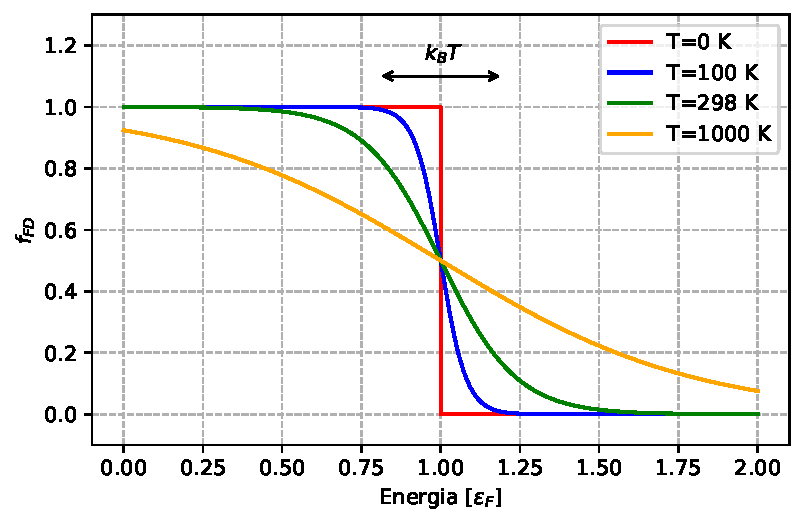
\includegraphics[scale=0.85]{Cuerpo/Append_A/Fermi-Dirac.pdf}
	\caption{Distribución de Fermi-Dirac.}
	\label{Fig:06-0}
\end{figure}    
Cuando $T\neq0$ la probabilidad de que este ocupado un estado de energía $\varepsilon>\varepsilon_F$ ya no es cero, de tal modo que el número de estados viene dado por:

\begin{equation}
	N=\int_{0}^{\infty} f_{FD}(\varepsilon,T) D(\varepsilon) \D \varepsilon \label{Ec:06-01-00}
\end{equation}
Si $T=0$ tenemos que la ecuación () se recupera verificándose que $\mu=\varepsilon_F$ dadas las definiciones previas. Sin embargo para temperaturas $T\neq 0$ no se verifica que sean iguales ($\mu(T\neq 0) \neq \varepsilon_F$). De hecho el valor de $\mu$ depende en última instancia de la ligadura (\ref{Ec:06-01-00}), de tal modo que para $T\ll T_F$ se verifica que:

\begin{equation}
	\mu(T) \approx \varepsilon_F \ccorchetes{1-\frac{1}{3}\parentesis{\frac{\pi T}{2T_F}}^2}
\end{equation}
que se deduce de la expansión de Sommerfeld.